\documentclass[11pt, a4paper]{article}
\renewcommand{\baselinestretch}{1.15} 
\usepackage[toc,page]{appendix}
\usepackage{mathptmx}
\usepackage[left=2cm,right=2cm, top=2cm, bottom=2cm]{geometry}
\usepackage{xcolor}
\usepackage{enumerate}
\usepackage[english]{babel}  % Caracteres en ESPAÑOL
\usepackage[utf8]{inputenc}
%\usepackage{authblk}
\usepackage{graphicx}
\usepackage{bigints}
\usepackage{multirow}
\usepackage{appendix}
\usepackage{hyperref}
\usepackage{apacite}
\usepackage{listings}
\usepackage{pdfpages}
\usepackage{subcaption}
\usepackage{verbatim}
\usepackage{amsmath,amsfonts,amssymb,amsthm,epsfig,epstopdf,titling,url,array}
\theoremstyle{definition}
\newtheorem{defn}{Definition}
\newtheorem{conj}{Conjecture}
\setlength{\arrayrulewidth}{1.5pt}
\begin{document}
%\title{Independent Study, Referee Report 2.a: \\ \textbf{Microeconomic Heterogeneity and Macroeconomic Shocks} \\ (Kaplan, \& Violante)}
%\author{Student: Christian Velasquez}
%\date{}
%\maketitle
\section{ECONOMY WITH DEFAULT}
	\subsection{SETTING THE MODEL:}
	The households maximize:
	\begin{equation}	
		E_0\left\{ \sum_t^{\infty} \beta^t U(c_t)\right\}
	\end{equation}
	The resource constrain is:
	\begin{center}
	\begin{equation*}
	 c = 
	 \begin{cases}
	 y + B - q(B',y)B' \quad \text{if repay}\\
	 y^{def}	 \text{\hspace{2.3cm} if they default}
	 \end{cases}
	\end{equation*}
	\end{center}
	Multiple risk neutral lenders in a competitive market, then by zero profits condition:
	\begin{equation}
		q(B',y) = \frac{1-\delta(B',y)}{1-r}
	\end{equation}
	The value function for a country with option to default:
	\begin{equation}
		v^o(B,y) = \max_{\{c,d\}}\left\{ v^c(B,y),v^d(y)\right\}
	\end{equation}
	where $v^c$ is the value of paying and $v^d$ is the defaulting value. Both are defining next:
	\begin{align}
	v^d(y) &= u(y^{def}) + \beta\int_{y'} \left[ \theta v^o(0,y') + (1-\theta)v^d(y')\right]f(y'|y)dy'\\
	v^c(B,y) &= max_{(B')}\left\{ u(y - q(B',y)B'+B) + \beta\int_{y'}v^o(B',y')f(y'|y)dy' \right\} 
	\end{align}
	In addition, countries face a borrowing constraint $B'\geq -Z$ to prevent Ponzi schemes. Let $A(B)$ and $D(B)$ be the repayment and default sets, such that:
	\begin{align}
	 A(B)&=\{y \in Y: v^c(B,y)\geq v^d(y)\}\\
	 D(B)&=\{y \in  Y: v^c(B,y)< v^d(y)\} 
	\end{align}
	Finally, the default probability is:
	\begin{equation}
		\delta(B',y) = \int_{D(B')}f(y'|y)dy'
	\end{equation}

	\subsection{RECURSIVE EQUILIBRIUM:}
	In this economy the equilibrium is a list of policy functions for consumption, debt, default a repayments sets, and bond prices such that:
	\begin{itemize}
		\item Taking as given everything else consumption maximize utility and satisfy resource constraint
		\item Taking as given the bond price; the policy function for debt $B'$ and sets $A(B)$ , $D(B)$ are in line with the government maximization problem
		\item Bond prices are consistent with the default set and the zero profit condition.
	\end{itemize}
	A clue to solve this model is to know that when $B=0$ the country is indifferent between defaulting or not, then $v^o=v^c=v^d$. The file $code1.jl$ solves the baseline model.
	\clearpage
	\subsection{RESULTS:}
	The solution has the form ($y_{low}\approx 0.95 E[y] ; y_{high}\approx 1.05 E[y]$):
%	\begin{figure}[!hbt]
%	\centering
%	\includegraphics[scale=0.5]{"./JuliaCode/Figures/Fig1.pdf"}\\
%	\includegraphics[scale=0.5]{"./JuliaCode/Figures/Fig2.pdf"}\\
%	\includegraphics[scale=0.5]{"./JuliaCode/Figures/Fig3.pdf"}
%	\end{figure}
	\clearpage
	\subsection{Simulation}
%	\begin{figure}[!hbt]
%		\centering
%		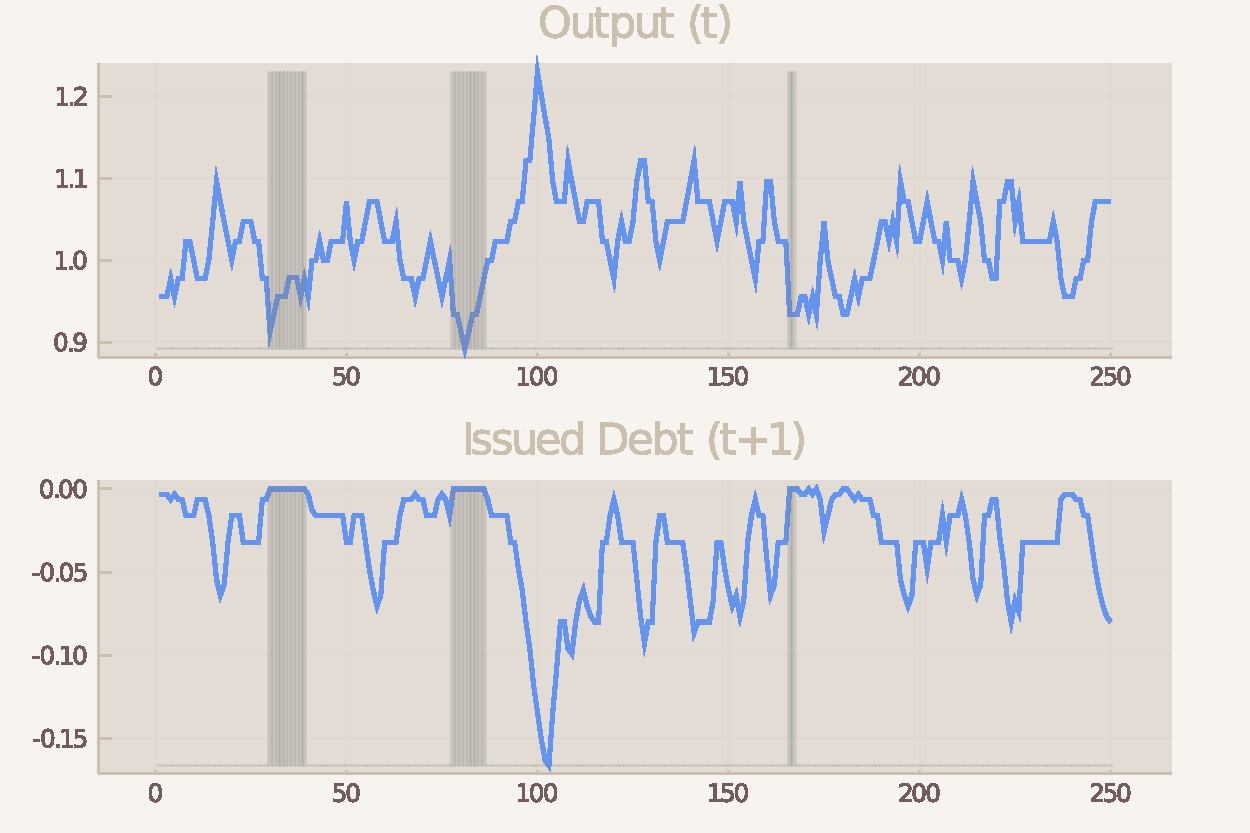
\includegraphics[scale=0.5]{"./JuliaCode/Figures/FigSim1.pdf"}\\
%		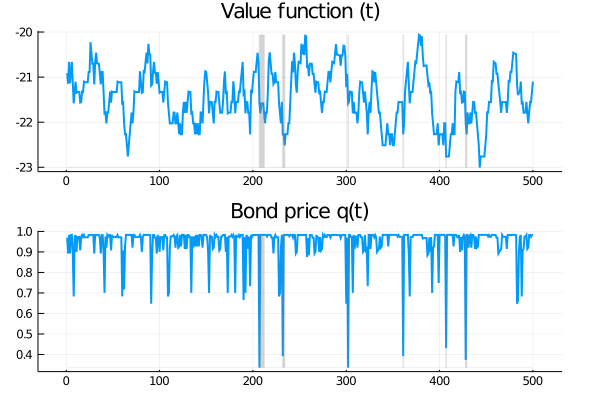
\includegraphics[scale=0.5]{"./JuliaCode/Figures/FigSim2.pdf"}\\
%		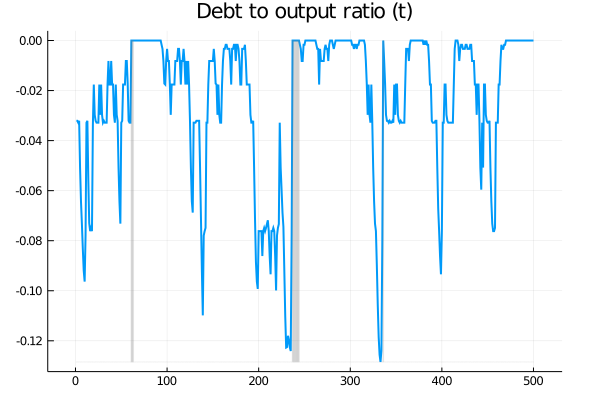
\includegraphics[scale=0.5]{"./JuliaCode/Figures/FigSim3.pdf"}
%	\end{figure}
	\subsection{NON LINEAR APPROXIMATION WITH NEURAL NETWORK}
	Following ..., I approximate the simulated value function and bond price with a neural network with one hidden layer with 16 nodes.
	\begin{equation}
		\hat{x}_t(s_t;\Theta) = \theta_0 + \sum_{q=1}^{Q} \theta_{q,1} \phi\left(\theta_{q,2}+\sum_{i=1}^{j}\theta_{q,2+i} \,\,s^{(i)}\right)
	\end{equation}
	The activation function is $\phi(k) = \log\left(1+e^{k}\right)$.\\
	First of all, I normalize all the states that are our inputs (let's $\tilde s$ the original variable):
	\begin{equation*}
		s_i := \frac{\tilde s_i - \frac{1}{2}(\sup(s)+\inf(s))}{\frac{1}{2}(\sup(s)-\inf(s))}	
	\end{equation*}
	The optimal $\Theta$ is chosen to minimize the sum of square residuals (I am assuming a univariate process):
	\begin{equation}
		\Theta =arg\,min_{\theta}\xi(\theta; s,\hat x) = arg\,min_{\theta}\frac{1}{2}\sum_{i=1}^{T}(x_i-\hat{x}_i)^2
	\end{equation}
	The first partial derivatives are (lets $e_i = x_i - \hat x_i$):
	\begin{align}
		\frac{\partial \mathcal{L}}{\partial \theta_0} &= -\sum_i e_i \\
		\frac{\partial \mathcal{L}}{\partial \theta_{j,1}} &= -\sum_i e_i \phi(k_{j,i}) \\
		\frac{\partial \mathcal{L}}{\partial \theta_{j,2}} &= -\sum_i \theta_{j,1} e_i \phi'(k_{j,i}) \\	
		\frac{\partial \mathcal{L}}{\partial \theta_{j,2+l}} &= -\sum_i \theta_{j,1} e_i \phi'(k_{j,i})s_{i,l}				
	\end{align}
	Then, the gradient is:
	\begin{equation}
		\theta_{m+1} = \theta_m - \epsilon_m \nabla_{\theta} \xi(\theta; s,\hat x)
	\end{equation}
	The minimization algorithm use a backtracking line search with a parameter $\gamma = 0.707$ (put a priori), hence
	\begin{align*}
		\text{while}&\\
		&\xi(x -\epsilon_{m,i}\nabla_\theta \xi(x))> \xi(x) - \frac{\epsilon_{m,i}}{2}\left(||\nabla_\theta \xi(x)||_2 \right)^2\\
		\text{then}&\\
		& \epsilon_{m, i+1} = \gamma \epsilon_{m,i} \\
		\text{leading:}&\\
		& \epsilon_{m}^* 
	\end{align*}
	therefore $\theta_{m+1} = \theta_m - \epsilon_m^* \nabla_{\theta} \xi(\theta; s,\hat x)$
	where $||\cdot||_2$ is the common Euclidean norm.
%	\begin{figure}[!hbt]
%		\centering
%		\includegraphics[scale=0.45]{"./JuliaCode/Figures/FigNR1.pdf"}
%		\includegraphics[scale=0.45]{"./JuliaCode/Figures/FigNR1b.pdf"}\\
%		\includegraphics[scale=0.45]{"./JuliaCode/Figures/FigNR2.pdf"}
%		\includegraphics[scale=0.45]{"./JuliaCode/Figures/FigNR2b.pdf"}
%	\end{figure}
\end{document}
